\documentclass[
	a4paper,
	12pt,
	oneside,
	titlepage,
	index=totoc,
%	halfparskip,
	chapterprefix,
]{scrbook}

\usepackage{typearea}
\usepackage[utf8]{inputenc}
\usepackage[english]{babel}
\usepackage[T1]{fontenc}
%\usepackage[sc]{mathpazo}
%\usepackage{tgpagella}
%\linespread{1.05} % Palatino needs more leading space between lines
\usepackage{graphicx}
\usepackage{color}
\usepackage{appendix}
%\definecolor{LinkColor}{rgb}{0,0,0.1}
\usepackage[
	pdfauthor={Klaus Trainer},
	pdftitle={Bachelor Thesis},
	pdfkeywords={CouchDB, Document-oriented Database, Quorum System, Reliability, Scalability},
	pdfsubject={Conception and Implementation of a Reliable Web Service with CouchDB}
]{hyperref}
\hypersetup{colorlinks=true,
    linkcolor=black,
    citecolor=black,
    filecolor=black,
    menucolor=black,
    urlcolor=black}

\usepackage{titlesec}
%% This gives us fun enumeration environments. compactenum will be nice.
\usepackage{paralist}

\usepackage{ctable}

\usepackage{tikz}
\usetikzlibrary{mindmap,backgrounds} % LaTeX and plain TeX
\usetikzlibrary[mindmap] % ConTeXt

\usepackage{listings}

\hyphenation{Erlang SEQUEL semi-struc-tured data-bases}

\titleformat{\chapter}
  {\normalfont\LARGE\bfseries}{\thechapter\hspace{1em}}{0pt}{}{}

\expandafter\def\expandafter\quote\expandafter{\quote\sffamily}

\makeatletter
\renewcommand\paragraph{
  \@startsection{paragraph}{4}{0mm}
    {-\baselineskip}
    {.5\baselineskip}
    {\normalfont\normalsize\bfseries}}
\makeatother

% An itemize-style list with little space between items
\newenvironment{innerlist}[1][\enskip$\circ$]%
        {\begin{compactenum}[#1]}{\end{compactenum}}

\nonfrenchspacing

\lstset{%
language=erlang,                % choose the language of the code
basicstyle=\footnotesize,       % the size of the fonts that are used for the code
numbers=left,                   % where to put the line-numbers
numberstyle=\footnotesize,      % the size of the fonts that are used for the line-numbers
stepnumber=2,                   % the step between two line-numbers. If it's 1 each line will be numbered
numbersep=8pt,                  % how far the line-numbers are from the code
backgroundcolor=\color{white},  % choose the background color. You must add \usepackage{color}
showspaces=false,               % show spaces adding particular underscores
showstringspaces=false,         % underline spaces within strings
showtabs=false,                 % show tabs within strings adding particular underscores
frame=single,	                % adds a frame around the code
tabsize=4,	                    % sets default tabsize to 2 spaces
captionpos=b,                   % sets the caption-position to bottom
breaklines=true,                % sets automatic line breaking
breakatwhitespace=false,        % sets if automatic breaks should only happen at whitespace
title=\lstname,                 % show the filename of files included with \lstinputlisting; also try caption instead of title
%escapeinside={\%*}{*)}          % if you want to add a comment within your code
%morekeywords={*,...}            % if you want to add more keywords to the set
}

%\setcounter{secnumdepth}{3}
%\setcounter{tocdepth}{3}


\begin{document}
\pagenumbering{Roman}
\begin{titlepage}

\flushright{
\includegraphics[width=216pt,height=51pt]{images/logo_fh}}

\vspace{10em}
\center

\Huge{\sf ''Conception and Implementation of a Reliable Web Service with CouchDB''}
\vspace{2em}

\Large{\sf
    by\\Klaus Trainer\\
}
\vspace{2em}
\Large{\sf
    in Partial Fulfillment of the Requirements for the Degree of\\
    {\bf Bachelor of Science in Computer Science}
    \vspace{2em}
    \\
    at the University of Applied Sciences Rosenheim\\
    Faculty of Computer Science\\
    \today
}
\vspace{3em}
\\
\Large{\sf
    Thesis Supervisors:\\
    Prof.\ Dr.\ Gerd Beneken and Prof.\ Dr.\ Dušan Petković
}

\end{titlepage}

\section*{Abstract}
This work is about developing a reverse proxy server for the document-oriented database \emph{CouchDB}. The objective is a web service that provides clients with the abstraction of a single reliable CouchDB device, using a collection of possibly unreliable CouchDB units. The main difference of the proposed solution in contrast to existing ones is that it selectively guarantees eventual or atomic consistency in the presence of concurrent data operations.

The purpose of this work is to facilitate the development of scalable CouchDB systems with guarantees on consistency, availability, and partition tolerance. Seth Gilbert and Nancy Lynch have proved that in an internet-scale distributed system it is possible to only guarantee either atomic consistency or availability. The interrelation between consistency, availability, and partition tolerance will be discussed with respect to practical tradeoffs.

Furthermore, with regard to the scalability of CouchDB applications, the need for data partitioning, load balancing, and clustering techniques as well as the resulting design considerations are discussed.

   Finally, an implementation of a reverse proxy that serves as an abstraction of a single reliable CouchDB device, will be proposed and evaluated.\\

\paragraph{Keywords}
CouchDB, Document-oriented Database, Quorum System, Reliability, Scalability

\section*{Acknowledgements}
Words fail to express my deep gratitude to my parents. Whatever road I would take, they have stood by me and supported me.\\

\noindent
Admittedly, I'm feeling a little bit like a dwarf standing on giants' shoulders. Thank you, giants, for sharing some of your farsightedness with me!\\

\noindent
Finally, I would like to thank everybody who has been a positive influence in my life.

\section*{Declaration}
I hereby state that this thesis was composed by myself, that the work contained herein is my own, except where explicitly stated otherwise in the text, and that this work has not been submitted for any other degree or professional qualification, except as specified.
\vspace{3em}\\
Rosenheim, \today \ \ \ \underline{ \ \ \ \ \ \ \ \ \ \ \ \ \ \ \ \ \ \ \ \ \ \ \ \ \ \ }\\
\hspace*{13.6em}\small{Klaus Trainer}

\tableofcontents
\listoffigures
\listoftables
\clearpage
\pagenumbering{arabic}
\chapter{Introduction}

\begin{quote}
{\itshape
The Internet and the Web did not have to exist. They come to us courtesy of misallocated defense money, skunkworks engineering projects, worse-is-better engineering practices, big science, naive liberal idealism, cranky libertarian politics, technofetishism, and the sweat and capital of programmers and investors who thought they'd found an easy way to strike it rich.
}

\hspace{1em}---Leonard Richardson and Sam Ruby \cite[p.~xviii]{RR07}\\
\end{quote}

\noindent
In a new era of media driven web applications, high concurrency, and global availability, companies are increasingly facing problems with upscaling databases to match the actual requirements.

Considerable research and effort has gone into developing the next stage of data storage solutions. For instance, several years ago, Google invested time and effort to figure out how to scale up their data operations \cite{CDG+08}. The result, named \emph{Bigtable}, was the product of research establishing that the way in which data for most Internet applications is used, does not meet the same original set of assumptions that went into the relational SQL\footnote{Structured Query Language; SQL was initially presented as ``structured English query language (SEQUEL)'' in \cite{CB74}.} databases designed in the 70's and 80's.

Researchers gained the fundamental insight that for most, but not all applications, multi-record locking mechanisms are not required, and key integrity can easily be managed on the application level. By designing a very simple columnar data system, it is possible to grow data operation to previously unheard dimensions.

Several years ago, Damien Katz, a former senior developer of the document management framework \emph{Lotus Notes}\footnote{\url{http://www.ibm.com/software/lotus/notesanddomino}}, saw the chance to take his experience with Lotus Notes, and what Google had accomplished with Bigtable, to merge the best features of both with each other. He started to develop \emph{CouchDB}\footnote{\url{http://couchdb.apache.org}}---a schema-less document-oriented database that leverages the distributed computability of Bigtable \cite[p.~8]{Cha09}.\\

\noindent
{\bf CouchDB.}
CouchDB is a schema-free document database server licensed under the Open Source Apache License, Version 2.0. It is accessible via an HTTP-based REST\footnote{Representational state transfer; the term describes an architectural style for distributed hypermedia systems. It has been introduced and defined in \cite[p.~76ff]{Fie00}. Architectures or interfaces conforming to the REST constraints are often referred to as being \emph{RESTful}.} application programming interface (API), and featuring robust, incremental peer-to-peer replication with conflict detection and management. It is also queryable and indexable (by creating \emph{Views}), featuring a table-oriented reporting engine that uses JavaScript as a query language.

CouchDB has been designed to efficiently support the quick development of document-centric web-based applications. The other major design goals are scalability (see definition in section \ref{Scalability}), and fault tolerance \cite[p.~4]{ASL10}. Because its design is based on simple, yet well understood core concepts, like e.g.\ HTTP, it should be easy to work with for people having experience with web technologies.

The central data structure in CouchDB are documents, which unlike in the relational data model, are basically self-contained units of data. The format in which documents are stored is JSON\footnote{JavaScript Object Notation; see \cite{rfc4627}}, which is natively compatible with JavaScript. It is possible to add attachments of any type (e.g.\ pictures, movies, or word documents) to a CouchDB document \cite[p.~41]{ASL10}. Because of all the properties mentioned before, CouchDB should be well-suited for document-centric web applications \cite[p.~4]{ASL10}.\\

\noindent
{\bf Erlang/OTP.}
CouchDB's implementation language is \emph{Erlang}, and the platform CouchDB has been built upon is \emph{OTP}\footnote{OTP (Open Telecom Platform) is a set of design patterns that support fault tolerance along with libraries that support those design patterns. For most applications, one would not implement any system in Erlang without using the OTP design principles and libraries \cite[p.~16]{LMC10}.}, which is included in any Erlang distribution.

Erlang/OTP is optimized for large scale, highly parallel and available, fault-tolerant applications \cite[p.~12]{Arm07} \cite{Eri09b}. Historically, it has been developed and used primarily at the Swedish telecom company \emph{Ericsson}, but since being publicly released under an Open Source License, it is facing increasing popularity within more and more other organizations \cite[p.~6f]{Arm03} \cite{Eri09a}.


\section{Motivation: Consistent CouchDB~Clusters}
\label{Motivation: Consistent CouchDB Clusters}

This work's motivation is to provide a technique that allows for the creation of CouchDB clusters that selectively guarantee eventual or atomic consistency of data. The purpose is to facilitate the creation of scalable CouchDB web services with guarantees on consistency, availability, and partition tolerance. To the author's best knowledge, no equivalent solution to this problem has been reported or previously recognized.

As the notion of \emph{scaling} (as well as its associated attributes \emph{scalable} and \emph{scalability}) has no generally applicable and accepted definition \cite{Hil90} \cite{DRW06} \cite[p.~145]{ASL10}, a definition that is coherent and valid, at least within the present context, is tried to be made in section \ref{Scalability}.\\

\noindent
{\bf Scaling CouchDB.}
To make a database system running on unreliable commodity hardware scalable, while maintaining certain guarantees on \emph{consistency}, \emph{availability}, and \emph{partition tolerance} (see section \ref{Consistency, Availability, Partition Tolerance}), techniques for \emph{data partitioning}, \emph{load balancing}, and \emph{clustering} are required. For a general definition and description of these techniques, see section \ref{Data Partitioning, Load Balancing, Clustering}. A detailed discussion of appropriate techniques and tools, with regard to the creation of a reliable web service with CouchDB, can be found in the problem analysis section (\ref{Problem Analysis}).


\section{Background}
\label{Background}

{\bf Riak.}
The database system that possibly shares the most similarities with CouchDB is \emph{Riak}\footnote{\url{http://riak.basho.com/}}. Riak was designed with decentralized clustering and partitioning support as primary features. For controlling the number of replicas within a cluster, there is a setting called the ``$N$ value'', which has a cluster-wide default, but can also be set on a per-\emph{bucket} (i.e.\ a collection of Riak objects) level.

The level of consistency among replicas is determined by the client. That is, for each read or write request the client has to supply an $R$ or $W$ value, respectively. The ``$R$ value'' represents the number of replicas that must report success before a write operation is considered complete. Accordingly, the ``$W$ value'' represents the number of replicas that must agree on an object to be retrieved \cite{Bas10a}.\\

\noindent
{\bf CouchDB Lounge.}
CouchDB Lounge is a proxy-based partitioning and clustering application for CouchDB \cite{Lou10a}. It contains \emph{dumbproxy}, which is a reverse HTTP proxy module for the web server \emph{nginx}\footnote{\url{http://nginx.org/}}. Dumbproxy manages database partitioning based on a consistent hashing algorithm \cite{Lou10b}, as well as replication. Documents will be replicated in bulk mode, i.e.\ when a certain (configurable) number of updates has accumulated, a replication request is added to a queue \cite{Lou10c}.\\

\noindent
As opposed to Riak, CouchDB has not been designed with decentralized clustering and partitioning support. However, as CouchDB's API is basically RESTful (see section \ref{RESTful HTTP Interface}), it is possible to provide those features in upper layers on top of CouchDB. It is the REST architectural constraints in particular that enforce the ability of building layered systems with RESTful architectures. CouchDB Lounge provides the very example for that.

CouchDB's push replication feature (see section \ref{Replication and Conflict Management}), as it is also used by CouchDB Lounge, can be used to build decentralized CouchDB clusters with each cluster node continuously replicating its changes to one or more other nodes, thereby guaranteeing \emph{eventual consistency} (see section \ref{Consistency}).

\chapter{General Principles and Concepts}

\begin{quote}
{\itshape
What you can do on one computer is limited, but what you can do with networks of computers becomes unlimited.
}

\hspace{1em}---Joe Armstrong, creator of the Erlang programming language \cite[p.~20]{Arm07}\\
\end{quote}

\section{Scalability}
\label{Scalability}

In section \ref{Motivation: Consistent CouchDB Clusters} it is mentioned that the notion of \emph{scaling} (as well as its associated attributes \emph{scalable} and \emph{scalability}) has no generally applicable and accepted definition \cite{Hil90}. In \cite[p.~145]{ASL10} it is explained that \emph{scaling} does not refer to a specific technique or technology. \emph{Scalability} is rather an attribute of a specific architecture that can vary for each system. According to Joe Stump, lead architect of \emph{Digg}\footnote{\url{http://digg.com}}, which is currently one of the internet's largest content aggregators, ``scaling is specialization'' \cite{Wat08}.

In \cite{DRW06} it is argued that, because of the ``intuitive notion that scalability is related to a system's ability to accommodate the `scaling' of some dimension [...] in a subjective field like scalability, a universal definition should be avoided''. In this context, ``a \emph{dimension} represents some aspects of the application domain (as defined by Jackson \cite{Jac95}) whose scaling affects system behavior''. To judge the extent of a system's scalability, ``stakeholders need a systematic way to understand causes, effects and their relationships''. A system then can be called \emph{scalable}, if it is possible ``to guarantee desired behavior when aspects related to the system vary''.\\

\noindent
{\bf Example: Determining CouchDB's Scalability.}
Since CouchDB is a database with a RESTful HTTP interface (see section \ref{RESTful HTTP Interface}), it basically provides two services: reads and writes.
Thus, there are three general properties that are key to scalability:
\begin{itemize}
	\item read requests
	\item write requests
	\item data.
\end{itemize}
\noindent
Unlike reads, writes are not cacheable. As a consequence, every write request hits the database's storage backend, which under high load, is most likely to become a bottleneck. Moreover, if multiple servers are used to speedup reads, a write must occur on all servers.

When the amount of data is more than a single server can make sensible use of, a solution is to chop the data into manageable chunks and put each chunk on a separate server \cite[p.~147]{ASL10}. This procedure is called \emph{data partitioning}.

Data partitioning can be used for scaling read/write requests as well as data. However, as the number of nodes in a distributed system increases, the system as a whole becomes increasingly prone to errors. Therefore, techniques for \emph{load balancing} and \emph{clustering} are needed. Explanations on data partitioning, load balancing, and clustering can be found in section \ref{Data Partitioning, Load Balancing, Clustering}.


\section{Consistency, Availability, Partition Tolerance}
\label{Consistency, Availability, Partition Tolerance}

\paragraph{The CAP Theorem}
In an invited talk at PODC 2000 \cite{Bre00}, Eric Brewer made the conjecture that it is impossible for a web service to provide the following three guarantees:
\begin{itemize}
	\item Consistency
	\item Availability
	\item Partition Tolerance
\end{itemize}
Just about two years later, the conjecture has been proved by Seth Gilbert and Nancy Lynch \cite{GL02}, and meanwhile, it is widely referred to as the \emph{CAP theorem}\footnote{\url{http://en.wikipedia.org/wiki/CAP_Theorem}}.

In their note, Gilbert and Lynch show that it is impossible to reliably provide atomic consistent data when there are partitions in the network. However, it is feasible to achieve any two of the properties: consistency, availability, partition tolerance. These properties, with regard to their respective tradeoffs, are explained in the remainder of this section.

\paragraph{Consistency}
\label{Consistency}
In transaction systems (the transaction model is explained in section \ref{Multiversion Concurrency Control}) the term \emph{consistency} is used to describe two different properties.

As defined in the ACID properties (atomicity, consistency, isolation, durability), it relates to failure atomicity and the guarantee that when a transaction is finished the database is in a consistent state.

The other consistency property that shall be explained here, does not describe states, but rather the order of concurrent data operations (i.e., \emph{serializability}, see section \ref{Multiversion Concurrency Control}).\\

\noindent
{\bf Sequential Consistency.}
\emph{Sequential consistency} was first defined by Leslie Lamport in \cite{Lam79} as a property that requires that
\begin{quote}
the result of any execution is the same as if the operations of all the processors were executed in some sequential order, and the operations of each individual processor appear in this sequence in the order specified by its program.
\end{quote}

That means that every node of the system sees data operations on the same data object in the same order, whereas the order may be different from the order as defined by the real time (as measured e.g.\ by a global physical clock) of issuing the operations. Instead of a total ordering of data operations, only a partial ordering is needed. The partial ordering is defined by the ``happened before'' relation, and can be imposed by the usage of logical clocks \cite{Lam78}.\\

\noindent
{\bf Atomic Consistency.}
\emph{Atomic consistency} (which is also referred to as \emph{strict} consistency) requires that data operations on a concurrently shared data object appear to be executed sequentially, i.e.\ every read always returns the most recently written value.

The notion of \emph{atomicity}, as a consistency property, was formalized in \cite{Lam86} on the basis of a shared data object stored in an

\begin{quote}
[...] \emph{atomic} register, which is safe and in which reads and writes behave as if they occur in some definite order. In other words, for any execution of the system, there is some way of totally ordering the reads and writes so that the values returned by the reads are the same as if the operations had been performed in that order, with no overlapping.
\end{quote}

Later, the corresponding correctness condition \emph{linearizability} was introduced by Herlihy and Wing \cite{HW87} \cite{HW90}. The idea of a consistent service can be expressed as the guarantee of linearizability for all read/write operations. 

In contrast to sequential consistency, where there has to be a partial ordering of data operations only, linearizability requires that data operations are totally ordered. A distributed algorithm for synchronizing a system of logical clocks, which can be used to totally order data operations, was first presented by Lamport in \cite{Lam78}.\\


\noindent
{\bf Other Consistency Models.}
In \cite{Lam86}, Lamport not only formalized the atomic consistency model, but also the weaker \emph{regular} and \emph{safe} consistency models. Their informal description is given as follows:

\begin{quote}
	The weakest possibility is a \emph{safe} register, in which it is assumed only that a read not concurrent with any write obtains the correct value---that is, the most recently written one. [...]

	The next stronger possibility is a \emph{regular} register, which is safe (a read not concurrent with a write gets the correct value) and in which a read that overlaps a write obtains either the old or new value.
\end{quote}

It is important to note that all of Lamport's consistency models will only hold for read/write storage abstractions with no partitioning network. That is, for any of these consistency models to hold, the communication links between the storage abstraction's base objects are not allowed to fail.

As soon as a distributed system is of internet scale, network partitions are a given, and hence it is not even possible to guarantee safe consistency. Nonetheless, for possibly partitioning distributed systems, other consistency models are needed. Consequently, Werner Vogels (Amazon CTO and Vice President) described, amongst other consistency models, \emph{weak consistency} and \emph{eventual consistency} \cite{Vog09}:

\begin{quote}
  \begin{itemize}
    \item \emph{Weak consistency}. The system does not guarantee that subsequent accesses will return the updated value. A number of conditions need to be met before the value will be returned. The period between the update and the moment when it is guaranteed that any observer will always see the updated value is dubbed the \emph{inconsistency window}.
    \item \emph{Eventual consistency}. This is a specific form of weak consistency; the storage system guarantees that if no new updates are made to the object, eventually all accesses will return the last updated value. If no failures occur, the maximum size of the inconsistency window can be determined based on factors such as communication delays, the load on the system, and  the number of replicas involved in the replication scheme.
  \end{itemize}
\end{quote}

\paragraph{Availability}
For a distributed system to be continuously available, every client (read/write) request received by a non-failing node in the system must result in a correct response. Modifying this condition to only require \emph{almost all} request to receive a response (i.e.\ probabilistic availability) does not change the result when arbitrary failures occur. For simplicity, one can require 100\% availability \cite{GL02}.

Obviously, the definition of availability does not contain an assertion about time. However, in practice, the notion of correct response is usually qualified by an upper time limit, i.e., any correct response must be received by the requesting client within bounded time. If no response is received within a certain period of time, there is no correct response by definition, which in turn means that the service is unavailable.

\paragraph{Partition Tolerance}
Availability and atomic consistency are qualified by the need to tolerate
network partitions. According to \cite{GL02}, ``In order to model partition tolerance, the network will be allowed to lose arbitrarily many messages sent
from one node to another''. When a network is partitioned, all messages sent
from nodes in one partition to nodes in another partition are lost. Any pattern
of message loss can be modeled as a temporary partition that separates the
communicating nodes at the moment of message loss.

The consistency requirement implies that every response will be of atomic consistency, although arbitrary messages that are sent might not be delivered.

The availability requirement implies that every client request received by a non-failing node in the system must result in a response, although arbitrary messages that are sent may be lost.

To summarize, partition tolerance means that ``No set of failures less than total network failure is allowed to cause the system to respond incorrectly'' \cite{GL02}.

\section{Data Partitioning, Load Balancing, Clustering}
\label{Data Partitioning, Load Balancing, Clustering}

In his book \emph{Programming Erlang} \cite[p.~175]{Arm07}, Joe Armstrong, creator of the Erlang Programming language, gives a summary of reasons for creating distributed programs:

\begin{quote}
  \begin{itemize}
	\item \emph{Performance}\\
	      We can make our programs go faster by arranging that different
	      parts of the program are run in parallel on different machines.
	\item \emph{Reliability}\\
	      We can make fault-tolerant systems by structuring the system to
	      run on several machines. If one machine fails, we can continue on
	      another machine.
	\item \emph{Scalability}\\
	      As we scale up an application, sooner or later we will exhaust
	      the capabilities of even the most powerful machine. At this stage
	      we have to add more machines to add capacity. Adding a new
	      machine should be a simple operation that does not require large
	      changes to the application architecture.
	\item \emph{Intrinsically distributed application}\\
	      Many applications are inherently distributed. If we write a
	      multiuser game or chat system, different users will be scattered
	      all over the globe. If we have a large number of users in a
	      particular geographic location, we want to place the computation
	      resources near the users.
	\item \emph{Fun}\\
	      Most of the fun programs that I want to write are distributed.
	      Many of these involve interaction with people and machines all
	      over the world.
  \end{itemize}
\end{quote}

Data partitioning, load balancing, clustering, and the cited reasons for creating distributed programs are very closely interrelated. While it is probably possible to have fun outside the world of distributed programming, performance, reliability, and scalability cannot be achieved without data partitioning, load balancing, and clustering techniques.\footnote{The question whether it is possible to create high-performance, reliable, and scalable programs without having fun, however, cannot be answered at this point. It has to be subject to further study.}

\paragraph{Data Partitioning}
{\bf Motivation.} Data partitioning solves the problem of having more data than a single device can hold. Aside from that, data partitioning is also a matter of performance optimization. Until solid-state drives (SSDs) will have replaced customary hard disk drives (HDDs), high seek times causing high latency (and definitively not the disk drives' sequential data throughput rate) are likely to be the limiting factor for overall data throughput.

In \cite{BBC+98}, Bernstein et al.\ noted with respect to that,
\begin{quote}
	while disk capacities are improving very quickly, seek times are improving relatively slowly. Hence, the amount of data that can be transferred to main memory during an average seek time is rising very quickly. Put differently, the cost of a seek relative to the transfer of a byte of data is rising quickly. This requires storage architectures that are much more serious about disk arm optimization. Also, ``arm wasting'' architectures, such as RAID 5, may be inappropriate in the future.
\end{quote}

Spreading different data records across several disk drives decreases the amount of concurrent read/write operations per disk under high load, and hence decreases the average seek time. As a consequence, overall data throughput is increased not only because more data records can be retrieved in parallel, but also through the reduced latency.\\

\noindent
According to \cite{NCWD84}, "Partitioning in database design is the process of assigning a logical object (relation) from the logical schema of the database to several physical objects (files) in a stored database". There are two classes of data partitioning techniques to differentiate:
\begin{quote}
	\emph{Vertical partitioning} subdivides attributes into groups and assigns each group to a physical object. \emph{Horizontal partitioning} subdivides object instances (tuples) into groups, all having the same attributes of the original object. We refer to the physical objects that are a result of vertical or horizontal partitioning as \emph{horizontal} or \emph{vertical} fragments.
\end{quote}

\vspace{0.5em}
\noindent
{\bf Vertical Data Partitioning.} In contrast to relational databases, document-oriented databases (see section \ref{Document-oriented Database}), which basically store semistructured data, by definition have no fixed schema. Hence, no uniform set of attribute types can be assumed, even if documents are of the same document type. As a consequence, it is impractical to do vertical data partitioning in document-oriented databases in most cases.

One exceptional case, in which it could be sensible to do vertical data partitioning, is the existence of special attributes that are already treated differently by the database system. For example, CouchDB has the ability to store document attachments. Document read operations only return a document's body and some of its metadata, whereas references are given to the corresponding attachments. More precisely, there is a metadata field containing a list of all document attachments' metadata including their identifier. Unlike document bodies, attachments need to be replaced in their entirety in order to modify them. In practice, document bodies tend to be quite small and accessed frequently, while attachments are orders of magnitude larger and accessed less frequently (and especially rarely for modification).

Different data properties and access patterns result in a significant discrepancy with regard to storage requirements. Therefore, it can well make sense to optimize in terms of different storage technologies (and hence storage locations). For example, document bodies are designated to be stored on a storage medium optimized for very frequent but small random read/write operations with low latency, while document attachments ought to be stored on a storage medium optimized for less frequent but larger read/write operations with high sequential throughput.\\

\noindent
{\bf Horizontal Data Partitioning.} A common technique used for horizontal data partitioning, which is implemented e.g.\ in Riak as well as CouchDB Lounge, is \emph{consistent hashing}\footnote{The concept of consistent hashing has been introduced in \cite{KLL+97}. See there for a more comprehensive description and definition.}.

Consistent hashing techniques make sure that each document is stored in a partition that can be statically determined. More precisely, the document identifier is used to compute a hash code. The range of the hash function is divided into equally-sized partitions (also referred to as virtual nodes), and each physical node is assigned one or more virtual nodes. For example, if the hash function's range is divided into 16 partitions and there are four physical nodes, four partitions are assigned to each physical node.

When the number of physical nodes needs to be increased (e.g.\ for load balancing reasons, or because storage volume is hitting a limit), each physical node that contains more than one virtual node can be split, so that virtual nodes become physical nodes. The number of physical nodes can grow up to the number of virtual nodes \cite[p.~166f]{ASL10} \cite{Bas10b}.

\paragraph{Load Balancing}
One goal of load balancing is to prevent that a single node in a distributed system receives so many requests that it becomes ``swamped''. Besides rendering a single node unusable, too many requests destined to one location can also cause network congestion and therefore a bad effect on nearby nodes \cite{KLL+97}.

Load balancing prevents swamping by equally distributing system load across several physical nodes. It therefore also increases a system's overall performance, because it is able to handle more concurrent requests. In that sense, data partitioning can also be seen as a load balancing technique.

In short, the goals of load balancing are \emph{availability} and \emph{performance}.\\

\noindent
{\bf Example: Using the Domain Name System for Load Balancing.} The probably simplest and most widely used load balancing technique in the internet makes use of a domain name system (DNS) property and implementation details.

The basic data element in the DNS is a resource record. For example, the resource record of the type \emph{Address} ($A$) maps between a domain name and an IP address. By specifying multiple $A$ records for a particular domain name, multiple IP addresses can be associated with one domain name. Therefore, requests to one domain name can be spread over many physical IP devices, which is load balancing.

When a DNS server receives a resolution request, it sends a list of all addresses associated with the particular domain name back to the requester. For each request, the server changes the order of the addresses supplied in the response, choosing the order randomly or in a sequential ``round robin'' fashion. Most clients usually use the first address in the list returned by the server, so by changing the addresses' order the server ensures that requests are equally distributed to multiple IP addresses \cite[p.~904f]{Koz05}.

The described load balancing approach implies that failover has to be implemented on the client side. In practice that means, when a failure occurs, the client will switch over to a different address under the same domain name to (hopefully) retrieve an available non-failing node, and retry the operation that has been aborted.

\paragraph{Clustering}
Clustering techniques abstract a set of functionally similar or identical machines, so that it operates as a single system.\footnote{Generally, it is helpful to know that in computer science the term \emph{clustering} is also used in a different way to describe a certain class of data mining techniques, which is no matter of interest in this work.} In that sense, data partitioning and load balancing can be considered as clustering techniques. The use of load balancing as a clustering technique is described e.g.\ in \cite{rfc1794}, where T.\ Brisco noted:
\begin{quote}
	Initially; ``load balancing'' was intended to permit the Domain Name
	System (DNS) [1] agents to support the concept of ``clusters'' (derived
	from the VMS usage) of machines -- where all machines were
	functionally similar or the same, and it didn't particularly matter
	which machine was picked -- as long as the load of the processing was
	reasonably well distributed across a series of actual different
	hosts.
\end{quote}

Brisco was hinting at the fact that the concept of \emph{clusters} goes back to the \emph{VAXclusters} system, which is ``a highly available and extensible configuration of VAX computers that operate as a single system. [...] The software is a distributed version of the VAX/VMS operating system that uses a distributed lock manager to synchronize access to shared resources'' \cite{KLS86}.

Goals behind clustering are to increase a system's overall availability, fault tolerance, and performance. Fault tolerance is achieved by the elimination of single points of failure. Availability is achieved by both hardware and data redundancy, as well as adequate techniques for load balancing and failover. Together with load balancing techniques, data redundancy in turn can be utilized to increase performance.

\chapter{Principles and Concepts Characteristic of CouchDB}

\begin{quote}
{\itshape
Django may be built {\bf\it for} the Web, but CouchDB is built {\bf\it of} the Web. I've never seen software that so completely embraces the philosophies behind HTTP. CouchDB makes Django look old-school in the same way that Django makes ASP look outdated.
}

\hspace{1em}---Jacob Kaplan-Moss, Django developer \cite{Kap07}\\
\end{quote}

\noindent
This chapter is intended to give some understanding of main principles and concepts CouchDB is built upon as well as the solution proposed in this work.

One feature that is essential for CouchDB's power, is its table-oriented reporting engine that builds \emph{views} based on dynamically, incrementally generated indexes. The feature is based on the \emph{MapReduce} concept. Because MapReduce and CouchDB views are neither directly relevant to the problem analysis, nor to the proposed solution, their description is omitted. Instead, refer to \cite{DG04} and \cite[p.~53ff]{ASL10}, respectively.


\section{Document-oriented Database}
\label{Document-oriented Database}

CouchDB is a document-oriented database. As opposed to relational databases, document-oriented databases do not store data in tables with uniform sized fields for each record. Instead, each record is stored as a document.\\

\noindent
{\bf Semistructured Data.}
Documents are self-contained units of data and do not have to adhere to a strict separately defined schema. Although a separate schema that places loose constraints on the data may exist, there is no need of a separation between the content's description and the content itself. Because of these properties, documents can be referred to as ``self-describing'' and characterized as \emph{semistructured data} \cite{Bun97}.

There are many forms of data where it would be difficult, or even impossible, to impose a structure on. The most immediate example of data that cannot be constrained by a schema is the World Wide Web \cite{Bun97}. It can be seen as an infinite distributed heterogeneous database. Its primary data format XML, which today is the most popular example of a semistructured data format, is reconciling the concepts of databases and (hypertext) documents \cite{Abi01}.\\

\noindent
{\bf Documents Instead of Rows.}
One of the most fundamental differences between SQL based databases and document-oriented databases is the fundamental unit of data. In SQL, the fundamental unit of data that is dealt with, is the \emph{row}. In a document-oriented database, there are no tables and hence no rows, but \emph{documents} instead. Each document is identified by a unique key.

In the specific case of CouchDB, any documents are JSON documents. Since JSON can express arbitrarily complex data structures, it does not make sense to conceptualize the information in terms of simple rows \cite[p.~14]{Cha09}.


\section{RESTful HTTP Interface}
\label{RESTful HTTP Interface}

Characteristic of CouchDB itself, as well as of systems built on top of CouchDB, is the RESTful HTTP Interface.

Representational State Transfer (REST) is an architectural style for distributed hypermedia systems. An architectural style is a named, coordinated set of architectural constraints \cite[p.~xvi]{Fie00}. Architectures or interfaces conforming to the REST constraints are referred to as being \emph{RESTful}.

REST evolved within the Internet Engineering Taskforce (IETF)\footnote{\url{http://www.ietf.org}} during the development of the Hypertext Transfer Protocol (HTTP/1.0) \cite{rfc1945}, and its extensions HTTP/1.1 \cite{rfc2616} and Uniform Resource Identifiers (URI) \cite{rfc2396}, as an idealized model of how the World Wide Web \emph{should work} \cite[p.~148]{Fie00}. The needs of an internet-scale distributed hypermedia system, like the World Wide Web, are met by enabling processing of actions by intermediaries, dynamic substitutability of components, and the caching and reuse of interactions.

According to Roy Fielding, who introduced and defined REST in 2000 \cite[p.~xvii]{Fie00},
\begin{quote}
REST emphasizes scalability of component interactions, generality of interfaces, independent deployment of components, and intermediary components to reduce interaction latency, enforce security, and encapsulate legacy systems.
\end{quote}

\paragraph{REST Architectural Elements}
Fielding defines a software architecture as ``a configuration of architectural elements---components, connectors, and data---constrained in their relationships in order to achieve a desired set of architectural properties'' \cite[p.~7]{Fie00}. He then defines the terms \emph{configuration}, \emph{component}, \emph{connector}, and \emph{datum} as follows \cite[p.~10ff]{Fie00}:
\begin{quote}
    A component is an abstract unit of software instructions and internal state that provides a transformation of data via its interface.[...]

    A connector is an abstract mechanism that mediates communication, coordination, or cooperation among components.[...]

    A datum is an element of information that is transferred from a component, or received by a component, via a connector.[...]

    A configuration is the structure of architectural relationships among components, connectors, and data during a period of system run-time.
\end{quote}

\begin{table}[h]\small
\begin{tabular}{l l}
\toprule[0.15em]
    {\bf Component}
    &{\bf Modern Web Examples}
\\\midrule[0.15em]
    {origin server}
    &{Apache httpd, CouchDB}
\\\midrule
    {gateway}
    &{CGI, reverse proxy (e.g.\ Squid, CouchDBCP)}
\\\midrule
    {proxy}
    &{Privoxy, Tinyproxy, Transproxy}
\\\midrule
    {user agent}
    &{cURL, Mozilla Firefox, Epiphany}
\\\bottomrule[0.1em]
\end{tabular}
\centering
\caption{REST Components (c.f.\ \cite[p.~96]{Fie00})}
\label{REST_Components}
\end{table}

\begin{table}[h]\small
\begin{tabular}{l l}
\toprule[0.15em]
    {\bf Connector}
    &{\bf Modern Web Examples}
\\\midrule[0.15em]
    {client}
    &{libcurl, lhttpc}
\\\midrule
    {server}
    &{Apache API, Mochiweb}
\\\midrule
    {cache}
    &{browser cache, Akamai cache network}
\\\midrule
    {resolver}
    &{bind (libresolv library), tinydns (djbdns library)}
\\\midrule
    {tunnel}
    &{SOCKS, SSL after HTTP CONNECT}
\\\bottomrule[0.1em]
\end{tabular}
\centering
\caption{REST Connectors (c.f.\ \cite[p.~93]{Fie00})}
\label{REST_Connectors}
\end{table}

\begin{table}[h]\small
\begin{tabular}{l l}
\toprule[0.15em]
    {\bf Data Element}
    &{\bf Modern Web Examples}
\\\midrule[0.15em]
    {resource}
    &{the intended conceptual target of a hypertext reference}
\\\midrule
    {resource identifier}
    &{URL, URN}
\\\midrule
    {representation}
    &{HTML document, JPEG image}
\\\midrule
    {representation metadata}
    &{Last-Modified, Content-Type}
\\\midrule
    {resource metadata}
    &{ETag, Alternates, Vary}
\\\midrule
    {control data}
    &{If-None-Match, Cache-Control}
\\\bottomrule[0.1em]
\end{tabular}
\centering
\caption{REST Data Elements (c.f.\ \cite[p.~88]{Fie00})}
\label{REST_Data_Elements}
\end{table}

The REST style is an abstraction of the architectural elements within a distributed hypermedia system. It focuses on the role of components, the constraints upon their interaction with other components, and their interpretation of significant data elements. The REST constraints define the basis of the web architecture, and thus the essence of the web's behavior as a network-based application \cite[p.~86]{Fie00}.

The tables \ref{REST_Components}, \ref{REST_Connectors}, and \ref{REST_Data_Elements} give a summary of the respective architectural elements.

\paragraph{REST Constraints}
REST places constraints on connector semantics, where in contrast other architectural styles enforcing distributed object access and RPC (Remote Procedure Call) mechanisms (for instance \emph{CORBA}\footnote{Common Object Request Broker Architecture; see \url{http://www.corba.org}}), have focused on component semantics.

The basic REST architectural constraints (cf.\ Sect.~5.1 \cite{Fie00}) are:
\begin{itemize}
	\item {\bf Client-Server} Architectural Style
	\item {\bf Stateless} Communication
	\item Client-side {\bf Cache}
	\item {\bf Uniform Interface} Between Components
	\item {\bf Layered System}.
\end{itemize}

At this point, only the stateless communication constraint will be discussed in detail, as it is strongly related to the other four constraints. A detailed explanation of all REST architectural constraints, as well as a description of the architectural elements and their interplay (i.e.\ architectural views), is given in chapter five of Fielding's dissertation \cite[p.~76ff]{Fie00}. For those who are interested in the subject's practical issues (e.g.\ design and implementation of web services, best practices), the book \emph{RESTful Web Services} \cite{RR07} could be a good source of information. Finally, it should be pointed out that REST itself does not represent an architecture, but rather a set of design criteria (i.e.\ an architectural style). In chapter four of \cite{RR07}, a concrete RESTful architecture, which in contrast to REST, is explicitly tied to the web, is introduced: the \emph{Resource-Oriented Architecture} (ROA).\\

\noindent
{\bf Stateless Communication.}
All REST interactions are stateless; session state is kept entirely on the client. Thus, a request is \emph{self-contained}, i.e., independently of any preceding requests. All of the information that is necessary for a connector to understand a request, is contained in the request.

According to \cite[p.~93]{Fie00}, this restriction accomplishes four functions:
\begin{quote}
1) it removes any need for the connectors to retain application state between requests, thus reducing consumption of physical resources and improving scalability;

2) it allows interactions to be processed in parallel without requiring that the processing mechanism understand the interaction semantics;

3) it allows an intermediary to view and understand a request in isolation, which may be necessary when services are dynamically rearranged; and,

4) it forces all of the information that might factor into the reusability of a cached response to be present in each request.
\end{quote}

In a nutshell, stateless communication induces the properties of \emph{visibility}, \emph{reliability}, and \emph{scalability} \cite[p.~79]{Fie00}. Visibility is facilitated, because a monitoring system does not have to look beyond a single request datum in order to determine the full nature of the request. Reliability is facilitated, because statelessness eases the task of recovering from partial failures \cite{KWWW94}. Scalability is facilitated, because not having to store state between requests allows the server component to quickly free resources, and further simplifies implementation, as there is no need to manage resource usage across requests.

Furthermore, because stateless communication allows each interaction to be independent of the others, there is no need for an awareness of the overall component topology, which would be an impossible task for an Internet-scale architecture, anyway. Components can either act as a destination or as a intermediary, determined dynamically by the target of each request. Therefore, RESTful web services may be implemented using a complex hierarchy of intermediaries and multiple distributed origin servers \cite[p.~99]{Fie00}.\\

\noindent
{\bf Example: CouchDB's RESTful HTTP Interface.}
CouchDB's REST API features basically three HTTP methods: {\tt GET}, {\tt PUT}, and {\tt DELETE}. As an example, if a request's target is a document, the individual methods feature the following semantics:

\begin{itemize}
	\item {\tt GET}: retrieve a document or document attachment.
	\item {\tt PUT}: create or update a document or document attachment.
	\item {\tt DELETE}: delete a document.
\end{itemize}  

The {\tt POST} method, amongst other things, is used to trigger replication. However, it cannot be spoken of as a part of the REST API, because it is not corresponding to REST, but to an RPC style instead \cite[p.~44]{ASL10}.

A detailed hands-on introduction to CouchDB's API can be found in chapter four of \cite{ASL10}, whereas the exhaustive API reference can be retrieved online\footnote{\url{http://wiki.apache.org/couchdb/Reference}}.


\section{Multiversion Concurrency Control}
\label{Multiversion Concurrency Control}

In this section the terms \emph{Concurrency Control} and \emph{Multiversion Concurrency Control}, as well as the respective correctness criteria, \emph{serializability} and \emph{one-copy serializability}, are explained. The goal is to give an idea of those concepts, to be able to understand the principles behind CouchDB's Multiversion Concurrency Control implementation. For exhaustive definitions and descriptions of those concepts see \cite{Pap79}, \cite{BG81}, and \cite{BG83}.\\

\noindent
{\bf Transactions.}
The unit of data processing in a distributed system is the \emph{transaction}. A transaction is a portion of a program that issues reads and writes to a database system (DBS). For concreteness, one can assume that each transaction is a process, and each data item is managed by a separate process. (However, the assumption is not required) \cite{BG82}. In addition, it is assumed that a transaction transforms a consistent state into a new consistent state.

A transaction's outcome can be that it has either \emph{aborted}, because an operation was rejected by the DBS for some reason, or that it has \emph{commited}, and all operations were executed successfully. In case of an abort, every involved data item is left in the same state as before the transaction. In short, a transaction appears to execute either completely (it is said to \emph{commit}) or not at all (it is said to \emph{abort}). This property is referred to as \emph{failure atomicity} \cite[p.~242f]{GR06}.\\

\noindent
{\bf Concurrency Control's Purpose.}
Concurrency Control (CC) solves the problem of synchronizing concurrently executing transactions on a shared database. When transactions execute concurrently, the interleaved execution of their reads and writes by the DBS can produce undesirable results. CC is the activity of avoiding such undesirable results \cite{BG82}.

According to \cite{BG81}, ``The correctness of a concurrency control algorithm is defined relative to users' expectations regarding transaction execution'', and there are two correctness criteria, whose realization is CC's  principal issue:
\begin{quote}
(1) users expect that each transaction submitted to the system will eventually be executed;

(2) users expect the computation performed by each transaction to be the same whether it executes alone in a dedicated system or in parallel with other transactions in a multiprogrammed system.
\end{quote}

\vspace{0.5em}
\noindent
{\bf Serializability.}
In accordance with the just illustrated correctness criteria, the goal of CC is to guarantee \emph{serializable} execution of transactions. Thus, the notion of correctness in this context is that of \emph{serializability}, which is attained by controlling the order in which reads and writes are processed \cite{Pap79} \cite{BG83}.

In \cite{BG81}, serializability has been described as follows:
\begin{quote}
Let $E$ denote an execution of transactions $T_1, ..., T_n$. $E$ is a serial execution if no transactions execute concurrently in $E$; that is, each transaction is executed to completion before the next one begins. [...] An execution is serializable if it is computationally equivalent to a serial execution, that is, if it produces the same output and has the same effect on the database as some serial execution.
\end{quote}

\paragraph{Single-version Concurrency Control}
When dealing with concurrent data operations, a DBS must, in order to preserve data consistency, prevent the modification of data items while being read, and vice versa, must prevent data items from being read while being modified. In single-version DBSs, this is achieved by maintaining \emph{locks} of the respective data items. Transactions trying to modify data items that are concurrently read by different transactions are blocked, until the locks on the respective data items are released. As a consequence, \emph{deadlocks} may occur. For an example, take two transactions, each with a lock whose release the other transaction is waiting for. This problem can be handled by either prevention, or detection and elimination (see \cite{BG81}).

Another problem becomes evident when a transaction has modified data items and, for some reason, fails to complete. In this case, data items are likely to be inconsistent. However, as stated before, an essential property of transactions is failure atomicity. To preserve this property, a transaction \emph{rollback} mechanism has to be established. In the case of a transaction abort, the data items' state before the transaction is restored by the rollback mechanism. In order to guarantee that rollbacks can be performed at any time (imagine a database recovery, succeeding a failure that occurred while transactions were being executed), the rollback mechanism has to be able to retrieve all required data from a durable \emph{transaction log}, which is maintained by a \emph{log manager} (see \cite[p.~493ff]{GR92}).

\paragraph{Multiversion Concurrency Control}
According to \cite{Sil82}, the concept of Multiversion Concurrency Control (MVCC) has been used as early as 1973 in a version of the Honeywell FMS system \cite{Hon73}, and was formalized in \cite{SLR76}. The first description of a MVCC algorithm that is known of, is Reed's multiversion timestamping algorithm \cite{Ree78}. However, the term ``Multiversion Concurrency Control'' itself initially appeared later, e.g.\ in \cite{Sil82}.

In a multiversion DBS, each write on a data item $x$, produces a new copy (i.e.\ a version) of $x$. Versions of $x$ are denoted by $x_i, x_j, ...$, where the subscript is the index of the transaction that wrote the version. Operations on versions are denoted $r_i[x_j]$ and $w_i[x_i]$. For each read on $x$, the DBS selects one of the versions of $x$ to be read. To execute a transaction $T_i$, a multiversion DBS must \emph{translate} the transaction's ``data item operations'' into ``version operations''. This \emph{translation} can be formalized by a function, which maps each write operation $w_i[x]$ into $w_i[x_i]$ and each read operation $r_i[x]$ into $r_i[x_j]$ for some $j$.

Since writes do not overwrite each other, and since reads can read any version, the DBS has more flexibility in controlling the order of reads and writes. In contrast to single-version CC, one-copy serializability (see below) can be achieved without locking when (logical) timestamps are used. Because it is not necessary for a read access to a data item to lock out writes to the data item, and vice versa, writes do not need to block reads. Therefore, MVCC can allow more concurrency than single-version CC \cite[p.~158]{Ree78} \cite{BG83}.\\

\noindent
{\bf One-Copy Serializability.}
In contrast to a single-version database, where CC correctness only depends on the order in which reads and writes are processed, in a multiversion database it depends on the translation as well as the order. The corresponding correctness condition for MVCC algorithms is \emph{one-copy serializability}: an execution of transactions in a multiversion database is one-copy serializable, if it is equivalent to a serial execution of the same transactions in a single-version database \cite{BG83}.\\

\noindent
{\bf Multiversion Timestamping.}
The earliest MVCC algorithm that is known of is Reed's multiversion timestamping algorithm \cite{Ree78}.

When it begins executing, each transaction is assigned a unique \emph{timestamp} $TS(i)$, which tells the \emph{logical time} at which the transaction began. The timestamps are assigned by a \emph{logical clock} (see \cite{Lam78}), and hence are strictly increasing. Each read/write operation carries a timestamp (that of the transaction that issued it), and each version carries the timestamp of the transaction that wrote it.

Operations are basically processed first-come-first-served, but the translation from data item operations to version operations makes it appear as if they were processed in timestamp order.

According to \cite{BG83}, the algorithm works as follows:
\begin{quote}
  \begin{enumerate}[(1)]
    \item $r_i[x]$ is translated into $r_i[x_k]$, where $x_k$ is the version of $x$ with largest timestamp $\leq$ $TS(i)$.

    \item $w_i[x]$ has two cases. If the DBS has already processed $r_j[x_k]$ such that $TS(k) < TS(i) < TS(j)$, then $w_i[x]$ is \emph{rejected}. Otherwise $w_i[x]$ is translated into $w_i[x_i]$. Intuitively, $w_i[x]$ is rejected if it would invalidate $r_j[x_k]$.
  \end{enumerate}
\end{quote}

\vspace{0.5em}
\noindent
{\bf Example: CouchDB's MVCC Implementation.}
\begin{figure}[ht]
	{\flushleft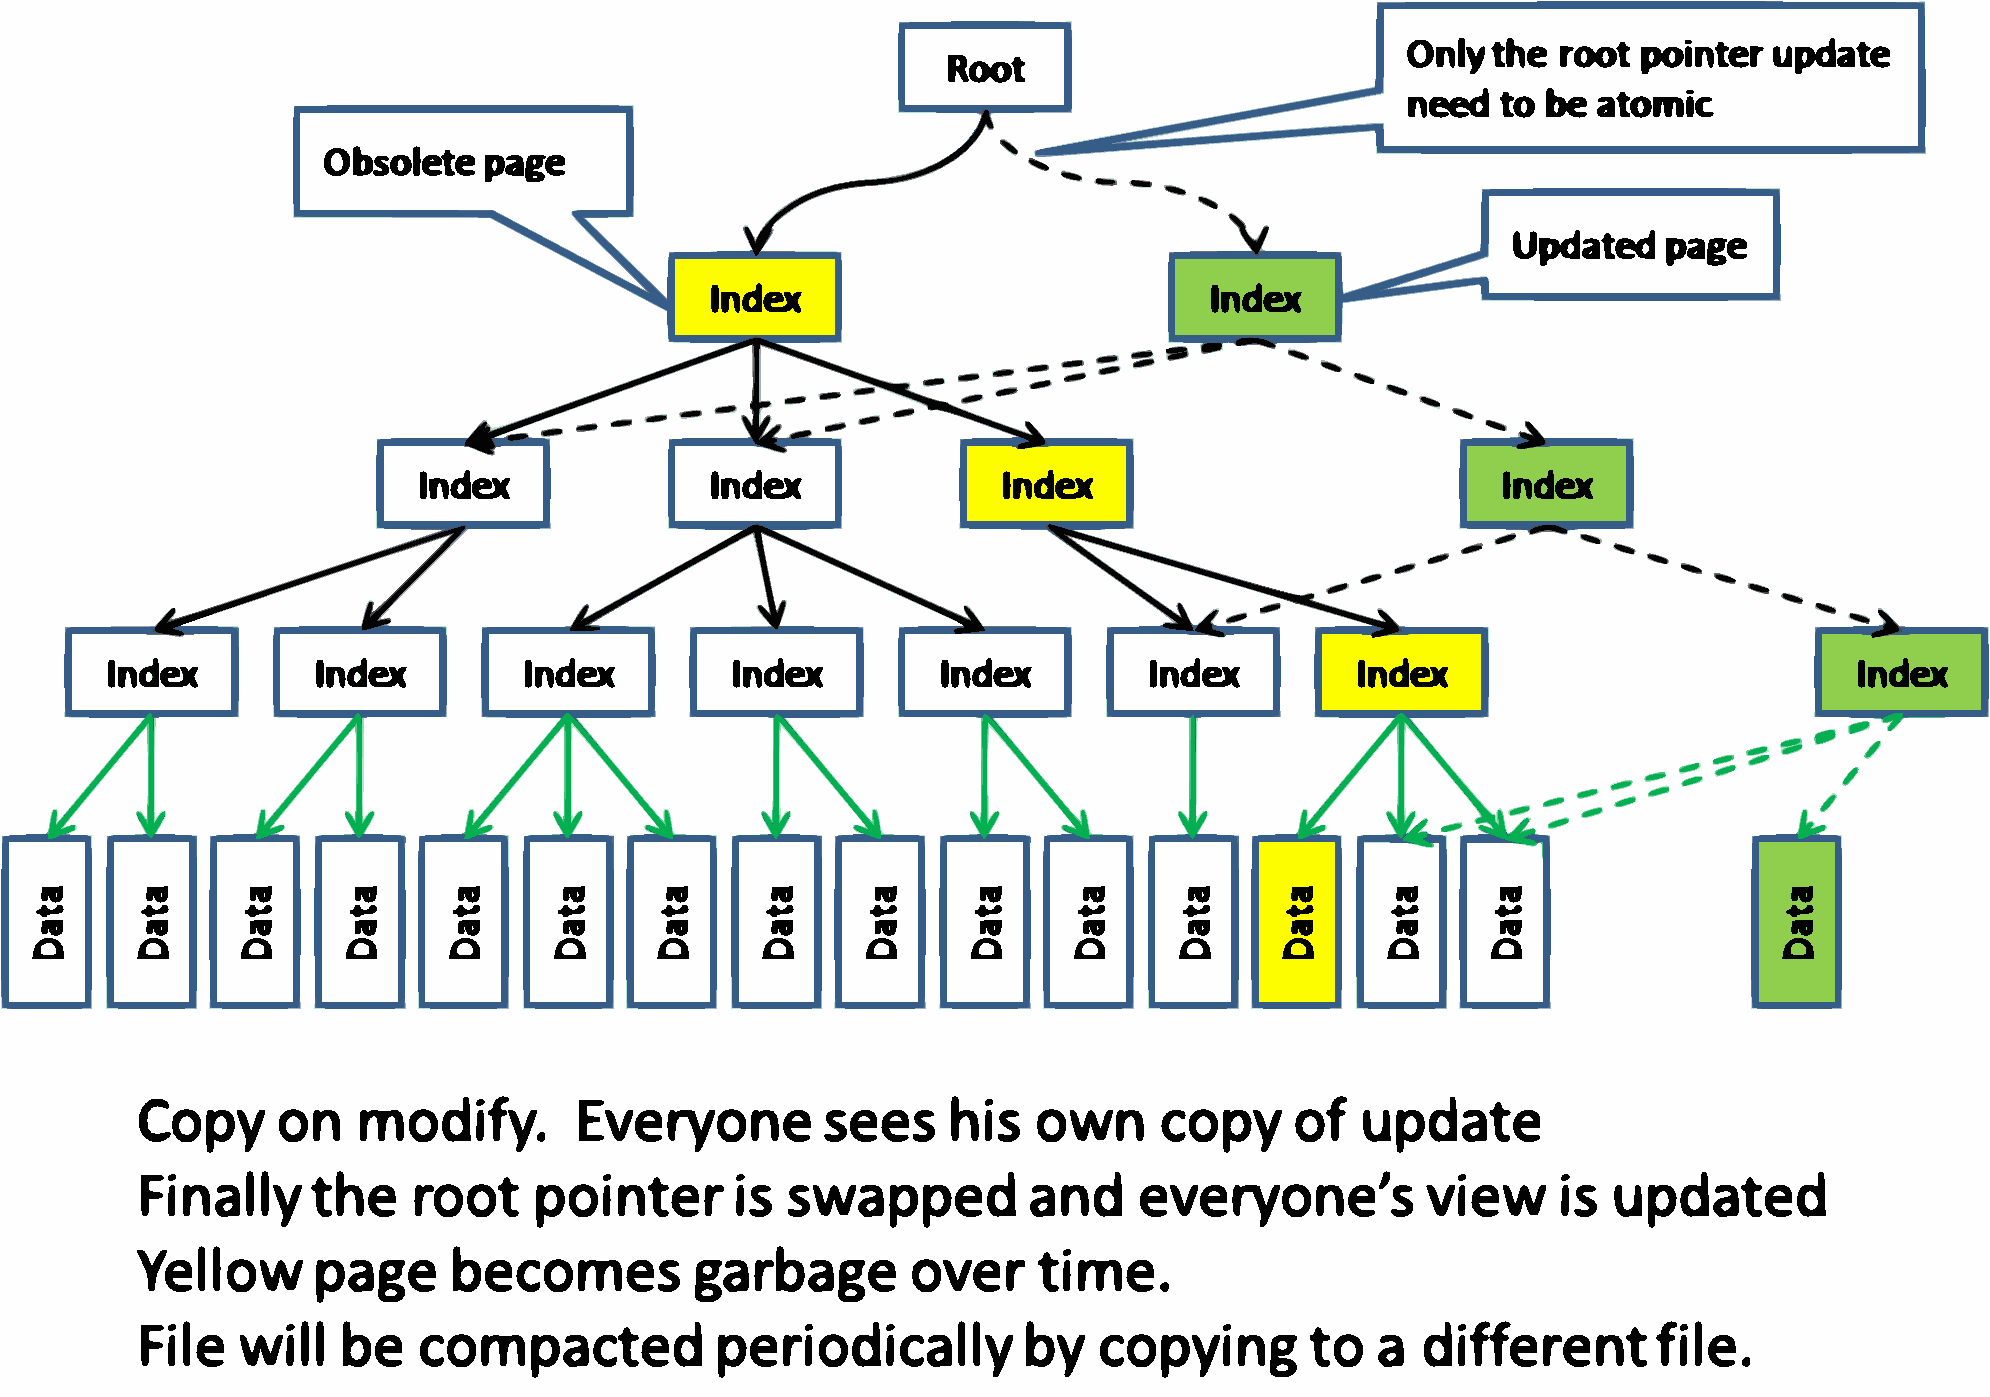
\includegraphics[width=\textwidth]{figures/MVCC}}
	\caption{CouchDB's MVCC index structure. Courtesy of Ricky Ho \cite{Ho09}.}
	\label{Ho09}
\end{figure}
CouchDB's MVCC mechanism ensures that, in case somebody else made a change unbeknownst to the updating client, its update will not be accepted. In order to update a document (that includes its deletion), the document's latest revision (i.e.\ version) number has to be specified in the respective request's query parameter {\tt rev}. (The concept behind CouchDB's revision numbers is explained comprehensively in section \ref{Replication and Conflict Management}.) The reason for that constraint is that it prevents clients from updating data they did not know existed. Simplified, it can be said that ``whoever saves a change to a document first, wins'' \cite[p.~39]{ASL10}.

To understand CouchDB's MVCC implementation, it is helpful to look at CouchDB's index structure. The data structure that is used to index documents and views is the $B^+$-tree.\footnote{Regarding the $B^+$-tree data structure, it is referred to \cite{Bay08} and \cite{Com79}.} For each database and for each view index, one $B^+$-tree is used. CouchDB's $B^+$-tree implementation features an append-only design. As illustrated in figure \ref{Ho09}, write-locks are only needed for one simple operation, namely for an update of the index's root pointer. Read-locks are not necessary at all.

Writes need to be serialized, so that for any single database only one write operation is allowed at any point in time. The reason is that for every write operation in a database, the $B^+$-tree's root node has to be rewritten in the database file. In doing so, like the $B^+$-tree, the database file is append-only as well. Old portions of the database file will never change, and every old $B^+$-tree root, in case that there are still references to it, will point to a consistent snapshot of the database.

Following from the described design, there can be any number of read operations at any given time, and each read operation is guaranteed a consistent view of the database.

For more details, e.g.\ on how failure atomicity and local data consistency are guaranteed at any time, see \cite[p.~233ff]{ASL10}.


\section{Replication and Conflict Management}
\label{Replication and Conflict Management}

{\bf Replication.}
CouchDB has a peer-to-peer replication feature that allows for uni- and bi-directional replication of any database changes. So it is possible to have several synchronized copies of the same database arranged in a decentralized fashion. Neither coordination of read/write operations nor central infrastructure is needed. Thus, the peer-to-peer replication feature allows for the creation of decentralized, eventual consistent CouchDB clusters.

The replication process, which is started by an HTTP {\tt POST} request, works incrementally. Only documents updated since the last replication are examined, and for each updated document only the changes are replicated. If replication fails, e.g.\ due to network problems or crash, the next replication restarts at the same document where it left off.

Replication can be triggered in two different modes: in pull mode it will be executed once, so that only the current changes will be replicated, in push mode not only the current changes but also future changes will be replicated continuously.

Furthermore, replication can be filtered by custom filter functions written in JavaScript or Erlang, so that only particular documents or those meeting specific criteria are replicated \cite[p.~149ff]{ASL10} \cite{Apa10}.\\

\noindent
{\bf Conflict Management.}
In CouchDB, conflicts are treated as a common state, not an exceptional one. Consequently, any number of conflicting document versions may exist in a database concurrently.

Each version (also referred to as \emph{revision}) of a CouchDB document has a deterministic unique revision history, which basically is an ordered list of the actual and all past revision numbers, stored in the document metadata. A particular document version can be retrieved by specifying its revision number in the respective HTTP {\tt GET} request as a value of the URL query parameter {\tt rev}. If the query parameter is not specified, the latest version is retrieved.

A conflict may occur when a document is replicated to a database. In particular, it occurs when two or more documents with the same identifier have a revision history that is of the same length, but the documents' revision histories or data differ. In this case, all conflicting document versions are stored, and each version is marked with a specific \emph{conflicts} flag.

In the presence of conflicts, some order between conflicting versions of a document needs to be established to decide over ``winning'' and ``losing'' versions. Except that only winning versions can appear in views, losing versions are just like any other version. They can be retrieved by specifying the revision number as a query parameter value and are also replicated.

A deterministic decentralized conflict management mechanism is important in a distributed system with redundant instances of the same database. Independently of the other instances' state or some other shared state (like e.g.\ chronological time), each instance is able to make deterministic decisions about the different versions' order.

When distributed update conflicts occur, all database replicas see the same winning revision, and each has the opportunity to resolve the conflict. Resolving conflicts can be done manually or, depending on the nature of the data and the conflict, by automated agents. Decentralized conflict resolution is possible while maintaining single document database semantics \cite{Apa10}.\\

\noindent
{\bf Deterministic Revision Numbers.} Revision numbers consist of an integer followed by a dash and a hash code: e.g.\ {\tt 3-5d0319b075a21b095719bc561def7122}. The integer is incremented for each new document revision and starts with the value $1$. The hash code is a md5 hash code over a set of document properties: the JSON body and some metadata fields. When there are conflicts, revision numbers are compared in ASCII sort order and the one with the highest ASCII values wins. Documents with the same content and revision history (and practically only those ones) have the same revision number and will not create any conflicts \cite[p.~153ff]{ASL10}.

A desired effect of this scheme is that it is deterministic and there is no need for shared state. This is also true for a distributed system, where for one version of a document there can be as many conflicting versions as the number of distributed nodes minus one. Take as an example that every node replicates its changes to every other node. Every node can make its conflict decision independently of the other nodes, without any shared state. Eventually (once each node has replicated its changes to every other node), all nodes will agree and expose the same view.

\chapter[Conception and Implementation of a Reliable Web Service with CouchDB]{Conception and Implementation of a\\Reliable Web Service with CouchDB}

\begin{quote}
{\itshape
Each node in a system should be able to make decisions purely based on local state. If you need to do something under high load with failures occurring and you need to reach agreement, you're lost. If you're concerned about scalability, any algorithm that forces you to run agreement will eventually become your bottleneck. Take that as a given.
}

\hspace{1em}---Werner Vogels, Amazon CTO and Vice President \cite[p.~13]{ASL10}\\
\end{quote}

\noindent
In chapter two, principles and concepts that generally apply to distributed systems have been explained. Principles and concepts that characterize CouchDB and make it especially well suited for the creation of reliable web services are presented in chapter three.

The goal of this chapter is to show how the principles and concepts CouchDB has been built upon, play nicely together, and almost predetermine how a reliable web service based on CouchDB ought to be implemented.

With regard to web services, the notion of reliability is defined as the ability to guarantee consistency, availability, and fault tolerance. In order to be able to maintain these guarantees, the concept of scalability (see section \ref{Scalability}) has to be included in the definition of web service reliability as well, in case that some aspects of a web service's application domain may scale to a larger size.


\section{Problem Analysis}
\label{Problem Analysis}

\paragraph{Research Method}
\begin{itemize}
	\item Identification and scope of the problem
	\item Critical literature review
	\item Establishment of the required terms and definitions
	\item Development of a model for reasoning, communicating, characterizing and predicting a CouchDB cluster's behavior
	\item Model implementation
	\item Model evaluation
\end{itemize}

\paragraph{Problem Statement}
As already mentioned in section \ref{Motivation: Consistent CouchDB Clusters}, this work's motivation is to develop a technique that allows for the creation of reliable CouchDB clusters that selectively guarantee eventual or atomic consistency of data.

The objective is a web service that provides clients with the abstraction of a single reliable CouchDB device, using a collection of possibly unreliable CouchDB units. Therefore, a scalable solution for CouchDB clusters that cannot only guarantee data consistency, but also availability and tolerance to several patterns of failure (e.g.\ crashes or network partitioning), shall be presented.

\paragraph{Scope of the Problem}
The relation between a reliable CouchDB web service and a CouchDB cluster is that a reliable CouchDB web service consists of a CouchDB cluster. The fact that a CouchDB cluster consists of several CouchDB devices, and, in turn, a CouchDB cluster is the abstraction of a single CouchDB device, means that clusters are composable, i.e.\ a CouchDB cluster can consist of several CouchDB clusters.

Hence, the problem of creating a reliable web service based on CouchDB can be reduced to the problem of creating a reliable CouchDB cluster, using data partitioning techniques as needed.

As already mentioned in section \ref{Background}, a solution for data partitioning exists with CouchDB Lounge. Because CouchDB Lounge is already documented elsewhere (see \cite{Lou10a} and \cite[p.~165]{ASL10}), there will be no further description at this point, as that would exceed the scope of this work.

\paragraph{Requirements}
\label{Requirements}
\noindent
{\bf Features and Functionalities.}
Figure \ref{mindmap_couchdb_cluster} shows features and functionalities (including their interrelation) that are needed to implement a reliable CouchDB cluster. Many of those are already part of CouchDB, or are part of existing standard architectural elements, i.e., components and connectors commonly used for providing web services. For instance, as described in the example from section \ref{Data Partitioning, Load Balancing, Clustering}, load balancing (including failover, but excluding health monitoring) can be handled by already existing connectors, namely DNS resolver and client.

The key feature to be implemented for CouchDB clusters has not been touched in previous work, at least not within that context, and was this work's initial motivation. It is the ability to choose between different consistency guarantees on a per-request basis. More precisely, it is desirable to be able to select the consistency guarantee that applies for a read/write operation when issuing the particular request.

A functionality that cannot be implemented in a generic way, is instance management. Its implementation would require knowledge of the actual hardware and software infrastructure the particular web service is deployed into. Therefore, it will not be discussed in this work.\\

\noindent
{\bf Architectural Requirements.}
Because reliability can only be achieved by avoiding single points of failure, the first architectural requirement is that of decentrality. For the sake of fault tolerance and availability, the architectural design must allow the usage of redundant instances of a component or connector, so that each instance is able to serve its purpose independently of the others.

The second architectural requirement is that components and connectors must conform to the REST constraints. As CouchDB follows the REST principles, it is advisable not to break the present architectural style when building on top of it. Accordingly, exceptions to that rule are allowed for the few cases where CouchDB itself is not RESTful.

\begin{figure}
	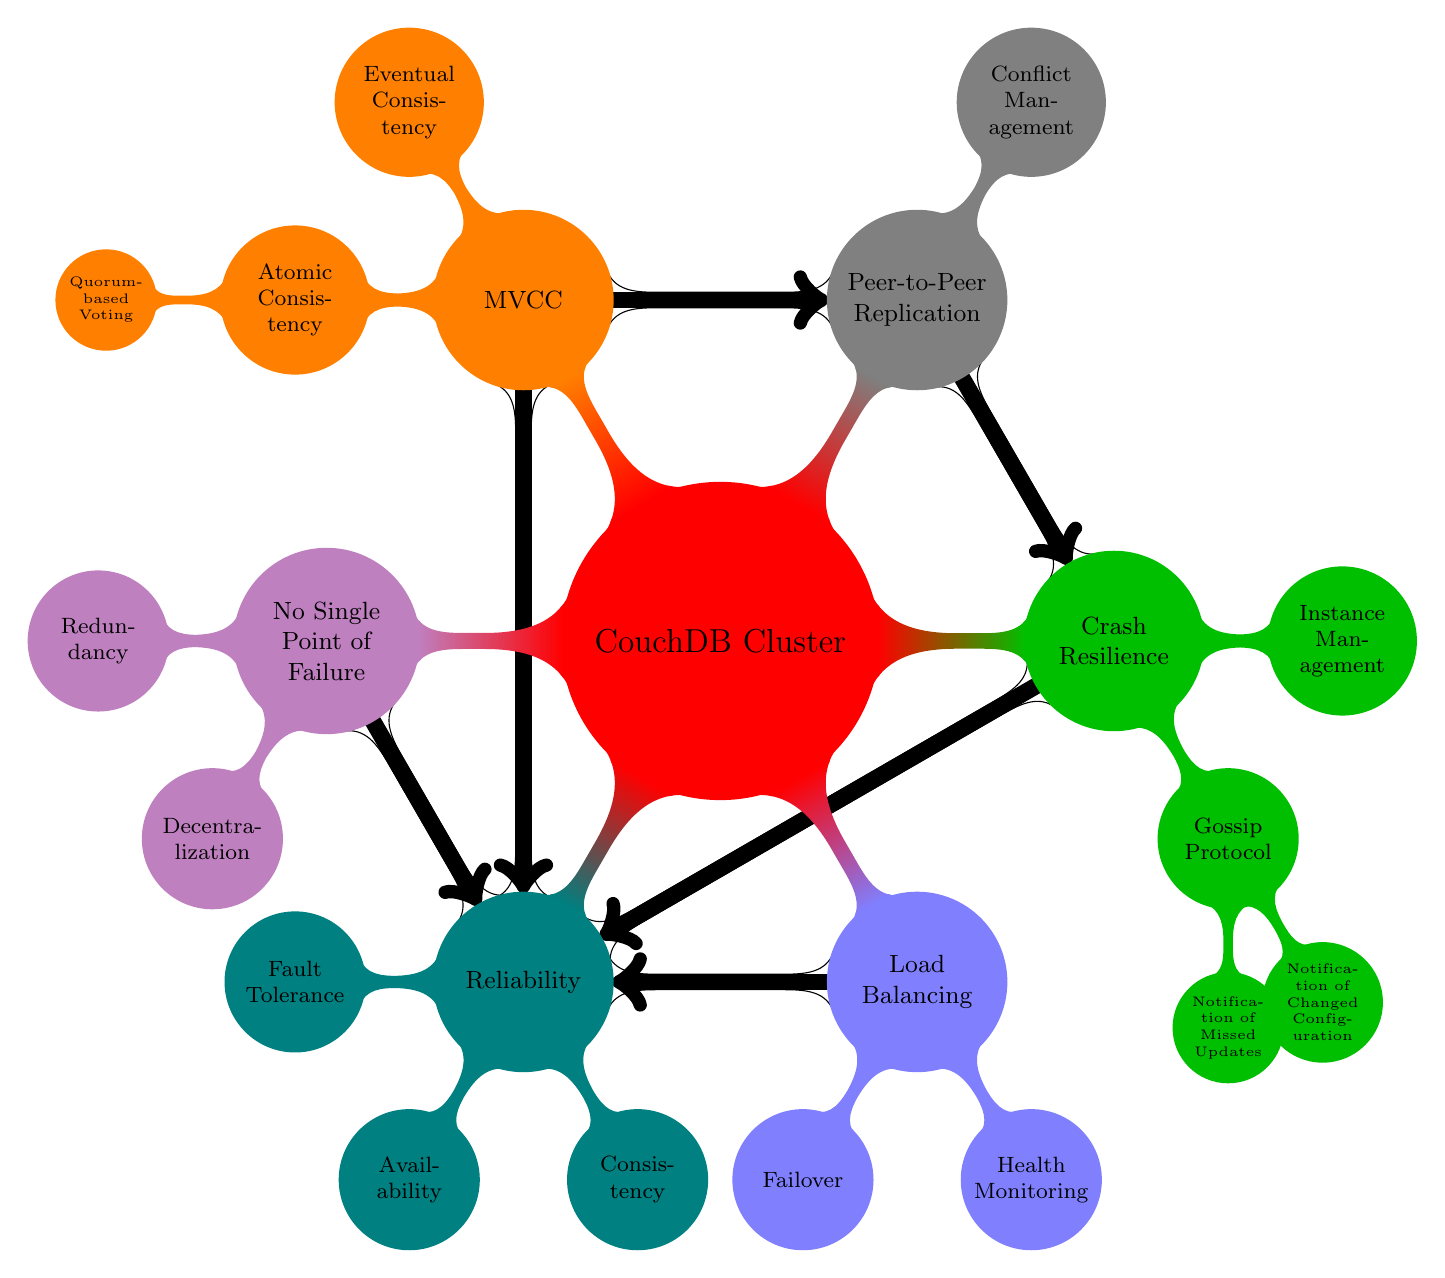
\begin{tikzpicture}
    \path[mindmap, concept color=red,text=black]
    node[concept] {CouchDB Cluster}[clockwise from=0]
    child[concept color=black!25!green] {
        node[concept] (res) {Crash Resilience}
        child[concept] { node[concept] {Instance Management} }
        child[concept] {
            node[concept] {Gossip Protocol}[clockwise from=-60]
                child[concept] { node[concept] {Notifica\-tion of Changed Configuration} }
                child[concept] { node[concept] {Notifica\-tion of Missed Updates} }
        }
    }
    child[concept color=blue!50] {
        node[concept] (loa) {Load Balancing}[clockwise from=-60]
        child[concept] { node[concept] (fai) {Health Monitoring} }
        child[concept] { node[concept] (fai) {Failover} }
    }
    child[concept color=green!50!blue] {
        node[concept] (rel) {Reliability}[clockwise from=-60]
        child[concept] { node[concept] {Consis\-tency} }
        child[concept] { node[concept] {Avail\-ability} }
        child[concept] { node[concept] {Fault Tolerance} }
    }
    child[concept color=violet!50] { 
        node[concept] (no) {No Single Point of Failure}[clockwise from=-120]
        child[concept] { node[concept] {Decentra\-lization} }
        child[concept] { node[concept] {Redun\-dancy} }
    }
    child[concept color=orange] {
        node[concept] (mvc) {MVCC}[clockwise from=180]
        child[concept] { node[concept] {Atomic Consistency}[clockwise from=180]
            child[concept] { node[concept] {Quorum-based Voting} }
        }
        child[concept] { node[concept] {Eventual Consistency} }
    }
    child[concept color=gray] {
        node[concept] (per) {Peer-to-Peer Replication}[clockwise from=60]
        child[concept] { node[concept] {Conflict Management} }
    };
    \begin{pgfonlayer}{background}
        \draw[circle connection bar switch color=from (white) to (black)]
            (per) edge (mvc);
        \draw[circle connection bar switch color=from (black) to (white)]
            (per) edge (res);
        \draw[circle connection bar switch color=from (white) to (black)]
            (rel) edge (res) edge (loa) edge (no) edge (mvc);
        \draw[<-, line width=6pt]
            (per) edge (mvc);
        \draw[->, line width=6pt]
            (per) edge (res);
        \draw[<-, line width=6pt]
            (rel) edge (res) edge (loa) edge (no) edge (mvc);
    \end{pgfonlayer}
\end{tikzpicture}

	\caption{Required Features and Functionalities of a Reliable CouchDB Cluster}
	\label{mindmap_couchdb_cluster}
\end{figure}


\section{System Model and Architecture}

\paragraph{System Model}
\label{System Model}
\begin{figure}
    \centering
	{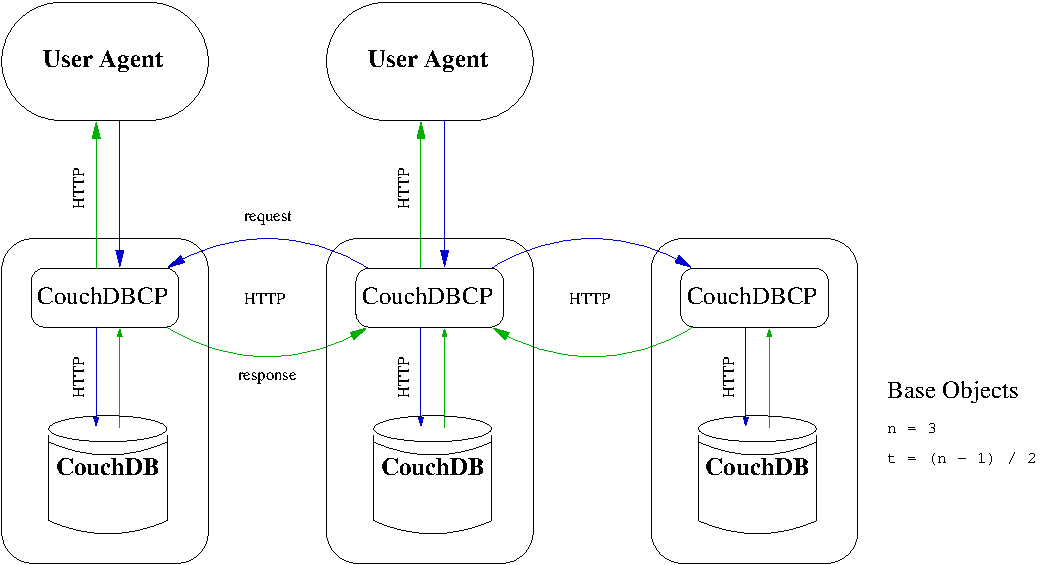
\includegraphics[width=\textwidth]{figures/system_components}}
    \caption{System Components}
    \label{system_model}
\end{figure}

Figure \ref{system_model} illustrates an example of a CouchDB cluster consisting of three identical (except for network configuration) base objects. Essentially, a base object consists of a CouchDB that is assigned to a \emph{CouchDBCP}\footnote{{\bf CouchDBCP} is an acronym for {\bf CouchDB} {\bf C}lustering {\bf P}roxy.}. A CouchDBCP is used as a gateway (more precisely as a reverse HTTP proxy) in front of a CouchDB. The two components are intended to be located nearby, connected with a high speed, low-latency network link; if not just simply located on the same computer. Client requests can be distributed across the base objects using load balancing techniques, like e.g.\ the one described in section \ref{Data Partitioning, Load Balancing, Clustering}. The CouchDBCP that receives a particular client request is referred to as the \emph{leader}.

In the example, there are two clients, each performing a data operation at the same time. The arrows indicate the HTTP requests and responses caused by the clients. The second client (from the left) has issued the request indicating that it needs to be served with atomic consistency guaranteed. The first client does not give such an indication, so that only eventual consistency semantics will be provided.\\

\noindent
{\bf Processes and Messages.}
The system's units that are able to perform computations are abstracted through the notion of \emph{process}, according to \cite[p.~26]{GR06}. The system is composed of a set of uniquely identified processes that know of each other, and run the same local algorithm. The sum of these copies comprises the actual distributed algorithm.

The processes communicate by exchanging uniquely identified messages, which are exchanged through communication \emph{links}.

For a more comprehensive and universal description of distributed computation abstractions, like processes and links, among other things, refer to \cite{GR06}.\\

\noindent
{\bf Automata and Steps.}
The distributed algorithm is viewed as a collection of distributed automata, one per process (c.f.\ \cite[p.~26ff]{GR06}). This goes back to Lamport \cite{Lam78}, who was first to use a sequential state machine implemented by a network of processors to describe the \emph{execution} of a distributed algorithm.

The automaton at a process regulates the way the process executes its computation steps, i.e., how it reacts to a message. A sequence of steps executed by the process represents the execution of a distributed algorithm. The elements of the sequences are the steps executed by the processes, whereas a finite sequence of steps represents a partial execution, and an infinite sequence of steps represents an infinite execution.

In the present model, the existence of a global clock provides a strictly increasing global notion of time that regulates the execution of the algorithms. The steps of the processes are executed according to ticks of the global clock, i.e., one step per clock tick. Although there may be several steps executed at the same physical instant, they are viewed as if they were executed at two different times of the global clock.

A process step (see figure \ref{step_of_a_process}) consists in \emph{receiving} a message from another process (global event), \emph{executing} a local computation (local event), and \emph{sending} a message to some process (global event). The algorithm, i.e., the process automaton, determines the execution of the local computation and the sending of a message. Local events that are generated are those exchanged between modules of the same process at different layers. It is important to notice that any interaction between local components of the same process, and with it, a message exchanged between modules of the very same process, is viewed as a local computation.

The fact that a process has no message to receive or send, or that there is no local computation to perform, is captured by the assumption that messages or computations might be $nil$.

For the present model, each base object is abstracted as one process; a CouchDBCP and its assigned CouchDB constitute one processing unit which can only fail as a whole. This simplification states that the units of a base object (i.e., a CouchDBCP and a CouchDB) are not physically distributed from each other. So, their exchanged messages are viewed as a interaction of modules of the same process, and hence as a local computation and not as a communication.\\

\begin{figure}
    \centering
	{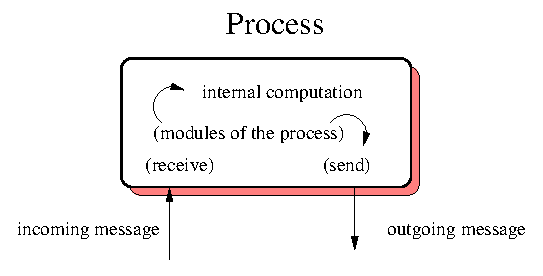
\includegraphics[width=150mm]{figures/step_of_a_process}}
    \caption{Step of a Process \cite[p.~27]{GR06}}
    \label{step_of_a_process}
\end{figure}

\noindent
{\bf Quorum Decisions.}
The problem of atomic consistency is solved by using \emph{quorums}. The first quorum system has been presented in \cite{Gif79} as a technique to maintain the consistency of replicated data. According to \cite{MR97},
\begin{quote}
    A well known way to enhance the availability and performance
    of replicated data is by using \emph{quorums}. A quorum system
    for a universe of servers is a collection of subsets of
    servers, each pair of which intersect. Intuitively, each
    quorum can operate on behalf of the system, thus increasing its
    availability and performance, while the intersection property
    guarantees that operations done on distinct quorums preserve
    consistency.
\end{quote}

From there, the correctness condition for quorum systems follows that if a quorum consists of $n$ processes, at least $(n / 2) + 1$ processes must be available.

In the present model, a quorum decision is defined as either the setting or the measurement of a global clock value. A global clock value exists, if there is a quorum of processes with a common logical clock value, i.e., a majority of processes have synchronous logical clocks.

Since in the system model, each process has a CouchDB instance as part of it, each process has its own logical clock. This is based on the fact that CouchDB's revision numbers are logical timestamps (i.e., they are strictly increasing). Basically, the multiversion concurrency control mechanism constitutes the logical clock, since it assigns the revision numbers; in other words, it provides the clock ticks.

Regarding quorum decisions, the following cases can be differentiated:
\begin{itemize}
    \item When a write operation has committed, a new global clock value was set, i.e., a majority of processes have advanced their logical clocks to the same value.
    \item When a read operation has committed, a global clock value could be measured, i.e., a majority of processes have synchronous logical clocks.
    \item When a data operation has aborted, no assertion can be made about clock synchronicity. Either there is no majority of processes with synchronous logical clocks (if so, the data would be inconsistent), or the data operation has aborted for some other reason (e.g., because the latest revision number was not specified in the write request).
\end{itemize}

\vspace{0.5em}
\noindent
{\bf Eventual Consistency.}
When only eventual consistency is guaranteed, a write request is forwarded by the leader to its assigned CouchDB, and as soon as the according response message has been received, the leader forwards it back to the requesting client. In case that the response message indicates that the write operation has been successful (i.e., it has committed), the written data is eventually replicated to all other base objects.

For read requests, the leader forwards the client's request to its assigned CouchDB, and again, forwards the according response message back to the client as soon it has been received.

For both read and write requests, if a leader has not received any response by its assigned CouchDB within a certain period of time, it sends the client a response with status code {\tt 503 Service Unavailable}.\\

\noindent
{\bf Atomic Consistency.}
In order to guarantee atomic consistency, the leader needs to interact with the other base objects. Each decision made by the leader has to be supported by a quorum of base objects.

When receiving a document read request (i.e.\ a {\tt GET} request), the leader sends a {\tt HEAD} request to the other CouchDBCPs as well as to its assigned CouchDB, in order to retrieve the document revision numbers from the particular CouchDBs. In the response messages, the document revision number is contained in the {\tt ETag} header field. When at least $(n / 2) + 1$ valid response messages (with status code {\tt 200 OK}) have been received, the revision numbers are compared in order to examine whether a quorum for some revision number exists. If that is the case, the leader requests the particular document version from its assigned CouchDB and forwards the response to the requesting client. Otherwise, i.e., if not enough valid response messages have been received, or if there is no quorum for any document version, a response with status code {\tt 503 Service Unavailable} is sent to the client.

When receiving a document write request, the leader forwards it to the other CouchDBCPs as well as to its assigned CouchDB. If at least $n / 2 + 1$ requests succeed, which can be detected by according responses with status code {\tt 201 Created}, one of those responses will be forwarded to the requesting client. Otherwise, a response with status code {\tt 503 Service Unavailable} will be sent.\\

\noindent
{\bf Recovery.}
The system's underlying abstraction for process failure is the crash-recovery abstraction described in \cite[p.~32ff]{GR06}.

A process is faulty if it either crashes and never recovers, or if it keeps crashing and recovering ad infinitum. Otherwise, if the process is always up and running, or if it crashes and recovers a finite number of times, it is correct (i.e., according to this abstraction of a process).

In the crash-recovery abstraction, processes can crash, which means the process stops sending messages, but might later recover. It should be noticed that accordingly, any pattern of message loss (e.g.\ due to network problems) is modeled as a process crash. The difference to an omission fault is that when a process crashes it might lose its internal state.

Figure \ref{failure_modes_of_a_process} depicts the different failure modes; the \emph{arbitrary fault} behavior is the most general one, while the \emph{crash failure}, which means that a process, once it has crashed, does never perform any computation (i.e.\ it does never recover), is the most specific failure mode (c.f.\ \cite[p.~29]{GR06}).

The recovery works as follows. When a write operation commits, the respective leader detects process crashes. If a process crash has been detected, the leader tells all available processes (including itself), to try to notify the crashed process about the missing update. This is what the processes then will do within random periodic time intervals. When the crashed process has eventually recovered, one of its peer processes will finally succeed to notify it about the missing update. Thereupon, the process will send an according read request to its peer processes in order to update the missing document version. Consequently, all peer processes receiving that read request will know that the crashed process has recovered and already been notified about the missing update, and therefore will stop sending any further notifications in this regard. 


\begin{figure}
    \centering
	{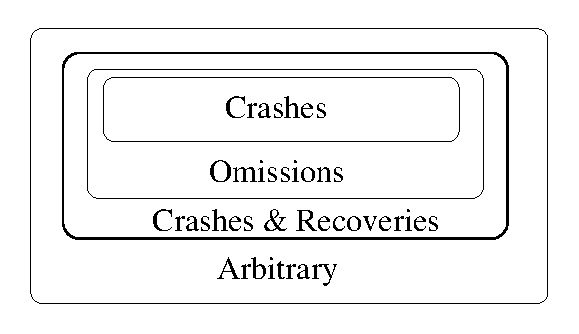
\includegraphics[width=100mm]{figures/failure_modes_of_a_process}}
    \caption{Failure Modes of a Process \cite[p.~30]{GR06}}
    \label{failure_modes_of_a_process}
\end{figure}

\paragraph{System Architecture}
Basically, the system architecture is quite simple. There is a decentralized, client-server style system with redundant CouchDBs, and a CouchDBCP used as a gateway in front of each CouchDB server.

This architecture allows for the achievement of this work's main goal---providing clients with the abstraction of a single reliable CouchDB device, while being able to choose between different consistency guarantees on a per-request basis---by just adding a connector.

The architectural requirements formulated in section \ref{Requirements} are met: there are no single points of failure, and the REST constraints that are kept by CouchDB are not violated.


\section{Correctness}
\noindent
{\bf Atomic Consistency.}
The atomic consistency of a standalone CouchDB instance follows intuitively from multiversion concurrency control (see section \ref{Multiversion Concurrency Control}). Atomic consistency is justified by the very fact that in any write request, clients need to specify the document's current revision number for the write operation to be successful. Therefore, it is impossible that a client overwrites a version whose existence it is not aware of. Moreover, the multiversion concurrency control makes sure that read and write operations are completely isolated from each other, i.e., only committed versions are available for read operations. As a result, all operations on a data object (in the present context a document) are arranged in a total sequential order. This corresponds to the definition of linearizability, which is the correctness condition for concurrently shared atomic data objects.

From the definition of a quorum (see section \ref{System Model}) follows that it is impossible to get more than one different quorum decision at the same point in time. Hence, it is impossible that different clients will succeed in writing different values concurrently, or that different values are returned to different clients' read requests concurrently. As any data operation depends on a quorum decision, this implies that the data operations are totally ordered.

Accordingly, Herlihy and Wing noted that linearizability is a \emph{local} property, which means that it is composable: ``a system is linearizable if each individual object is linearizable. Locality enhances modularity and concurrency, since objects can be implemented and verified independently, and run-time scheduling can be completely decentralized'' \cite{HW87}.\\

\noindent
{\bf Recovery.}
The recovery model is based on the correctness condition for quorum systems, which says that at any time a majority of processes (at least $(n / 2) + 1$) is available, and that base objects eventually recover and cannot be replaced by different processes. In addition, it is assumed that processes recover in the same order they fail, so that the first process that fails is the first one to recover.

As long as these conditions are fulfilled, i.e., if the system behaves correctly, any crashed process, as soon as it has recovered, will eventually be notified about updates it has missed.


\section{Implementation Aspects}

A CouchDBCP prototype has been implemented in Erlang/OTP, using the Mochiweb library as a server connector.

In order to support the cluster-specific semantics, custom header fields are used in the HTTP messages. For example, a CouchDBCP needs to be able to know whether a write request it received was issued by a client or by a CouchDBCP peer. In case the write request was issued by a client, the CouchDBCP would become the leader for that request. In that case, as a leader, it would perform different actions than it would perform as a non-leader.

If a client wants to change the (configurable) default consistency level for a particular request, it sets an accordant field (e.g.\ {\tt X-CouchDBCP-Consistency: atomic}) in the HTTP request header.

A detailed explanation and analysis of the implementation would exceed the scope of this work, and moreover, does not make a lot of sense at this early stage of implementation.

For a small piece of example code from the implementation, see the code listing that is provided in the appendix. The example code is a function that returns the first response from a list of responses to an HTTP {\tt HEAD} request, for whose {\tt ETag} header field value (which is the respective document's revision number) a quorum can be formed. In the case that no quorum can be formed, an error code is returned.


\section{Evaluation}

The prototype that has been developed contains several bugs. Features that are critical in production environments are missing. However, the prototype serves well for demonstration purposes and as a basis for further development. It has been tested being configured for atomic data consistency in a cluster consisting of three base objects; more than half of CouchDB's test cases passed successfully. The goal of developing a prototype that shows that the developed system model forms a valid basis for a practical implementation has been achieved.

The choice to use Erlang/OTP as a programming platform turned out to be a good one. Apparently, Erlang/OTP was designed for such or similar application domains, and hence it can be spoken of as the right tool for that purpose.

In particular, it is Erlang's inherent distributed programming abstractions (most notably processes and asynchronous messaging) that alleviate the development of highly concurrent, fault tolerant distributed programs. To highlight an example, Erlang's processes are extremely cheap with regard to their processing overhead and memory usage. It is possible to have ten-thousandths of processes running in parallel without having a significant decrease on system performance \cite[p.~148ff]{Arm07}.

Erlang discourages the use of shared memory, and mutable data objects in general, but instead encourages the use of high-level programming abstractions, generic design patterns (i.e., OTP \emph{behaviors}, see \cite{LMC10}), and also the use of parallel processes as many as needed, together with asynchronous message passing.

During the prototype implementation, none of Erlang/OTP's approaches revealed any downsides, even though some concepts were new to the author and had to be learned. In fact, the use of Erlang/OTP seems to result in fewer code, faster development, and less bugs, if compared to more mainstream programming platforms, like e.g.\ Java, applied to the same application domain.

\chapter{Conclusion}

\begin{quote}
{\itshape
Dealing with failure is easy: Work hard to improve. Success is also easy to handle: You've solved the wrong problem. Work hard to improve.
}

\hspace{1em}---Alan Perlis \cite{Per82}\\
\end{quote}

\noindent
This work's probably most significant result is that it shows how a reliable web service with atomic data consistency can be easily composed from RESTful base objects that use multiversion concurrency control.

However, there is still a lot of work to be done to make CouchDBCP mature enough to be usable in production systems. Once this has been achieved, there should be a good starting point to include data partitioning support, so everything that is necessary to scale CouchDB web services would be made available in one component.

Moreover, it will be interesting to discover further systems and application domains where principles and concepts described in this work can be applied, in order to develop similar solutions to the same problems. Conversely, there are systems, for instance Riak, that are subject to further study, in order to learn from their solutions to problems such as health monitoring or data partitioning.

\appendix
%\chapter{Example Code}
\chapter*{Appendix: Code Listing}
\label{Appendix}
\addcontentsline{toc}{chapter}{Appendix: Code Listing}
\chaptermark{Appendix}
\markboth{Appendix}{Appendix}

\begin{lstlisting}[caption=An Erlang function to find the first response for whose {\tt ETag} header field value (which is a document revision number) a majority exists.]
find_read_quorum(Responses, N) ->
    case lists:dropwhile(
        fun(E) ->
            {RespCode, ETag, _Header, _Proxy} = E,
            case lists:filter(
                fun(E1) ->
                    {RespCode1, ETag1, _, _} = E1,
                    case RespCode1 of
                    RespCode when ETag1 =:= ETag ->
                        true;
                    _ ->
                    false
                    end
                end, Responses) of
            L when length(L) =< N div 2 -> true;
            _ -> false
            end
        end, Responses) of
    [] ->
        {error, 503};
    [H|_] ->
        case H of
        {undefined, undefined, _Header, _Proxy} -> {error, 500};
        _ -> H
        end
    end.
\end{lstlisting}

\newpage
\bibliographystyle{alpha}
\bibliography{references}
\addcontentsline{toc}{chapter}{Bibliography}

\end{document}
